% \documentclass[10pt, english, pdftex]{template/UC3M_document}
\documentclass[10pt, spanish, pdftex]{template/UC3M_document}

%%%%% Preamble %%%%%
\author{Alejandro Prieto Macías}         % This is me! You should write here your name (for PDF metadata)
%%%%% About the authors (will be used on title page and header) %%%%%

%%% Indicate the number of authors by uncommenting the right option.
 \authorstwotrue     % 1 or 2 authors
% \authorsthreetrue   % 3 authors
%\authorsfourtrue    % 4 authors

%%% Fill with the authors data. You can leave empty keys {} if you need to and also if you provide more info that number of authors indicated it will be ignored.
% If you selected \authorstwotrue or \authorsthreetrue (1 to 3 authors)
\authorsuptothree{Alejandro Prieto Macías}{NIA 100383428}{Gr. 81}{Alejandro Valverde Mahou}{NIA 100383383}{Gr. 81}{Name3 Lastname3}{NIA 100XXXXXX}{Gr. XX}
% If you selected \coauthorsfourtrue (4 authors)
\authorsfour{Name1 Lastname1}{NIA 100XXXXXX}{Name2 Lastname2}{NIA 100XXXXXX}{Name3 Lastname3}{NIA 100XXXXXX}{Name4 Lastname4}{NIA 100XXXXXX}{Group XX}

%%% If you want to show coauthors email address on the title page, uncomment \emailtrue. Comment it otherwise.
%\emailtrue
% You can leave empty keys {} if you need to and also if you provide more info that number of authors indicated or \emailtrue is commented it will be ignored.
\emails{email1@domain.tld}{email2@domain.tld}{email3@domain.tld}{email4@domain.tld}


%%%%%%%%PARA EL mybox%%%%%%%%%%%%%%%%%%%%%%%%%%%%%%%%%%%%%%%%%%%%%%%%
% Cuadros de colores
\usepackage{tcolorbox}
\usepackage{wrapfig}

\newtcolorbox{boxAntonio}[2]
{colback=#2!5!white,colframe=uc3mDarkBlue,fonttitle=\bfseries,title=#1, flushleft title, width=\linewidth, height=5.7cm}
\newtcolorbox{boxSara}[2]
{colback=#2!5!white,colframe=uc3mDarkBlue,fonttitle=\bfseries,title=#1, flushleft title, width=\linewidth, height=4.8cm}
\newtcolorbox{boxCarla}[2]
{colback=#2!5!white,colframe=uc3mDarkBlue,fonttitle=\bfseries,title=#1, flushleft title, width=\linewidth, height=6.15cm}
%%%%%%%%PARA EL mybox%%%%%%%%%%%%%%%%%%%%%%%%%%%%%%%%%%%%%%%%%%%%%%%%


%%%%% Basic data about the document (Degree, subject, title, campus, page number custom text) %%%%%
\documentdata{Ingeniería Informática}{Interfaces de Usuario}{Práctica Final}{Leganés}{}

%%%%% Page style %%%%%
\header
\footer
\pagestyle{fancy}


\begin{document}
%%%%% Page title %%%%%
\titleMain

%%%%% Index %%%%%
\begin{spacing}{0.5}
    % \shipout\null                   % Blank page before index (after title page)
    \hypersetup{linkcolor=black}    % References/links on the index will remain black color
    \tableofcontents\newpage        % Index of the document
    % \listoffigures\newpage          % Index of pictures
    % \listoftables\newpage           % Index of tables
\end{spacing}


%%%%% DOCUMENT CONTENT %%%%%
\section{Definición del Prototipo}\label{prototipo}
Durante la realización del proyecto, hemos intento atenernos al máximo al diseño realizado en el prototipo.
En algunos casos se ha seguido feacientemente, pero en otros se ha modificado para adaptarlo a un diseño que correspondiese con alguna heurística o patrón con el fin de mejorarlo. En otros casos, por estética o funcionalidad hemos decido adoptar otro estilo. En cualquier caso, el estilo básico y estructural se ha mantenido en todo momento.

\subsection{Colores}
Uno de los primeros pasos fue la elección de colores que siguieran la estética del club al que representa el sitio web, pero siguiendo los principios de usar tres colores básicos y dos extra que deriven de ellos. Para ello, hemos usado href{}{software externo} para la creación de la paleta.









%%%%%%%%%%%%%%%%%%%%%%%5

\subsection{Objetivo}
El objectivo de este ejercicio es diseñar una plataforma para seguir e informarse sobre las actividades del \href{http://www.cplmadrid.com}{club de hockey CPL Madrid}.

\subsection{Conoce al Usuario}
Es importante definir a los posibles usuarios de la plataforma. Para ello vamos a modelizar a tres de ellos: un padre, un jugador y un posible inversor interesado en el equipo.

\subsubsection{José Antonio}
\begin{boxAntonio}{}{blue}
  \begin{wrapfigure}{l}{0.2\textwidth}
  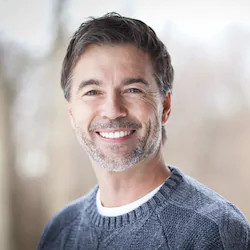
\includegraphics[scale=1.5]{Images/Antonio.jpg}
  \caption{José Antonio}
  \end{wrapfigure}
  \small José Antonio es un hombre de 45 años que tiene dos hijos que juega en el club CPL Madrid. En un entusiasta del hockey y le gusta seguir las ligas tanto de su hijo, como la de su hija. Este año le ha tocado ser el delegado del equipo de su hija, el equipo Benjamín. Por lo tanto, le toca subir las crónicas de los partidos en la página web del equipo. No se maneja demasiado bien con las tecnologías y por eso necesita que la web sea sencilla y fácil de usar. El móvil no es una herramienta para él, por eso prefiere revisar los partidos desde el PC del trabajo. También, necesita saber donde está la información que incumbe a los partidos de sus hijos, para saber cuándo y a dónde les tiene que llevar a jugar. \break
  Como siempre dice José Antonio:
  \textbf{"Con trabajo, trabajo, trabajo y mucho esfuerzo, se consiguen los sueños."}
\end{boxAntonio} \hfill \break

\subsubsection{Sara}
\begin{boxSara}{}{blue}
 \begin{wrapfigure}{l}{0.2\textwidth}
 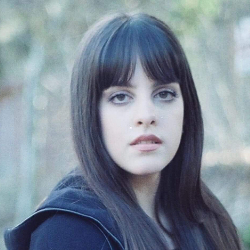
\includegraphics[scale=1.5]{Images/Sara.jpg}
 \caption{Sara}
 \end{wrapfigure}
 \small Sara es una joven de 17 años que juega en el club CPL Madrid en la sección femenina, Walkyrias. Es una chica un poco pasota, no tiene mucho interés en el resto de sus compañeras. Pero le encanta ver las estadísticas de sus temporadas anteriores, pues ya lleva 8 en el club, y ver que siempre ha estado la primera. Se pasa el día pegada al smartphone, cuando tiene partido lo consulta desde ahí para decírselo a sus padres. Puesto que le tienen que llevar al campo en coche.
 No tiene lema personal, pero siempre dice que \textbf{es la mejor}.
\end{boxSara}

\subsubsection{Carla}
\begin{boxCarla}{}{blue}
  \begin{wrapfigure}{l}{0.2\textwidth}
  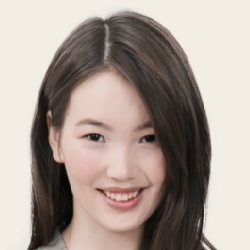
\includegraphics[scale=1.5]{Images/Carla.jpg}
  \caption{Carla}
  \end{wrapfigure}
  \small Carla es una joven emprendedora que trabaja para una compañía grande de móviles, y le han encargado que consiga que algún club deportivo de la Comunidad de Madrid lleve el logo de la empresa en la camiseta a modo de promoción. Carla ha encontrado de casualidad el sitio web del CPL Madrid. Ella busca un club ganador para poder llegar a la máxima cantidad de personas y con suerte aparecer en un periódico nacional. En el sitio web lo que quiere saber es la clasificación que ha conseguido el equipo en los últimos años. También necesita saber como ponerse en contacto con el club, además de su historia y que es lo que hacen. Carla trabaja a través de múltiples dipositivos: su smartphone, su tablet y su portátil. Lleva toda su vida usando las tecnologías, y está muy familiarizada con ellas.
  Carla solo tiene una cosa en mente, conseguir el puesto de CEO de la empresa trabajando desde abajo. En sus redes sociales siempre tiene de estado \textbf{"Go big or go home"}.
\end{boxCarla}

%Fin de sección de Usuarios
\pagebreak

\subsection{Entorno}
Para este apartado se han buscado sitios web de clubes grandes de los que conocemos que su diseño nos parece correcto para proceder con su análisis. Esto será de gran utiliadad para el desarrollo de nuestra propia aplicación, en este caso del sitio web que debemos renovar.
\subsubsection{Sitio web actual de \href{http://www.cplmadrid.com/}{CPL Madrid}}
En primer lugar, hemos analizado las funcionalidades de la propia web que debemos renovar.
\paragraph{Heurística de Nielsen}
\begin{itemize}
  \item \textbf{Visibilidad del estado del sistema}

  El sistema informa, a través de la barra de navegación, de la posición del usuario. Además, al visitar una subsección aparece un \textit{rastro de miga de pan}.

  \item \textbf{Coincidencia entre el sistema y el mundo real}

  El sistema no posee herramientas en las que exista coincidencia con el mundo real.

  \item \textbf{Control y libertad de los usuarios}

  El sistema no proporciona herramientas para regresar al estado anterior en caso de error o equivocación, más allá de la barra de navegación en algunos casos.

  \item \textbf{Consistencia y estándares}

  El sitio web no sigue las reglas de consistencia llegando a utilizar diferentes estilos e incluso duplicando las herramientas navegación.

  \item \textbf{Prevención de errores}

  No posee un sistema de prevención de errores. Tampoco es necesario puesto que la interacción del usuario simplemente es navegar por las distintas páginas.

  \item \textbf{Minimizar la carga de la memoria del usuario}

  El sistema no obliga al usuario a recordar cómo usar el sitio. La navegación resulta intuitiva.

  \item \textbf{Flexibilidad y eficiencia de uso}

  La diferencia entre un usuario nuevo y uno experimentado no es grande, pero el experimentado podría encontrar apartados con mayor agilidad.

  \item \textbf{Diálogos estéticos y diseño minimalista}

  El diseño es antiguo, poco cuidado e inconsistente.

  \item \textbf{Ayudar a los usuarios a reconocer, diagnosticar y recuperarse de los errores}

  No posee tampoco un sistema de recuperación de errores, pueden resultar inesperados y la solución es ir atrás con los botones propios del navegador.

  \item \textbf{Ayuda y documentación}

  Tampoco cuenta con ayuda ni documentación extra.
\end{itemize}
\paragraph{Patrones de Diseño de Van Duyne}
  \begin{itemize}
    \item \textbf{A12: Blogs}

    El sitio web tiene una estructura de blog porque tiene diferentes entradas organizadas en una lista.
    La aplicación cumple con el patrón de diseño de mantener la página como algo personal, y que permite los comentarios de los usuarios.
    Por el contrario, no cumple el hacer sencillo encontrar la información, ya que está muy desorganizado, y no posee ningún filtro.

    \item \textbf{B8: Páginas organizadas por categoría}

    El sitio web está organizado por categorías, porque cada pestaña de la aplicación constituye un apartado diferente completamente del resto.
    Aunque está organizado de esta forma, no cumple los patrones de diseño necesarios, ya que no usa un \textit{layout} consitente, ya que el formato cambia entre pestañas. Tampoco mantiene el método de navegación, ya que, dependiendo en el apartado en el que se encuentre el usuario, la barra de navegación cambia de diseño y de posición. Solo informa de la posición del usuario en algunas de las categorías, usando títulos resaltados.

    \item \textbf{E5: Sobre nosotros}

    El sitio web posee de un apartado de \textit[Conócenos], donde aparece toda la información relevante del club de hockey.

    \item \textbf{I6: Consistencia en el contenido de los \textit{sidebar}}

    En casi todas las pesañas de la apliación aparecen unas \textit{sidebar} con contenido que puede ser interesante para los usuarios en todo momento. Esto facilita el acceso de los usuarios. Su posicionamiento se mantiene siempre a la derecha de la página, y tienen siempre la misma longitud, que es menor al tamaño máximo del sitio web.

    \item \textbf{J1: Búsqueda de acciones dentro de la página}

    El sitio web cuenta con un buscador con herramientas de búsqueda de \textit{Google}. Está colocado en una posición visible: En la parte superior de la página.

    \item \textbf{K2: Barra de navegación}

  \end{itemize}

\subsubsection{Sitio web del \href{https://www.atleticodemadrid.com/}{Atlético de Madrid}}
En segundo lugar, nos ha parecido oportuno optar por revisar la web de este club puesto que sabemos que tiene caracterísitcas que podían ser útiles.

\paragraph{Heurística de Nielsen}
\begin{itemize}
  \item \textbf{Visibilidad del estado del sistema}

  El sitio muestra el título de la sección visitada. Además, de un \textit{rastro de miga de pan}, pero no resulta claro.

  \item \textbf{Coincidencia entre el sistema y el mundo real}

  El sistema no posee herramientas en las que exista coincidencia con el mundo real.

  \item \textbf{Control y libertad de los usuarios}

  El sistema proporciona libertad y control satisfactorio de la web. A excepción, de algunos casos que debido al formato de la pantalla no se pueden visitar.

  \item \textbf{Consistencia y estándares}

  El sitio web mantiene un estilo constante y no varía en función de la acción que el usuario esté haciendo.

  \item \textbf{Prevención de errores}

  En el caso de que el usuario quiera comprar una entrada y se equivoque de partido, no hay manera de retornar a la lista de partidos teniendo que cerrar la pestaña del navegador.

  \item \textbf{Minimizar la carga de la memoria del usuario}

  El sistema no obliga al usuario a recordar cómo usar el sitio. La navegación resulta intuitiva.

  \item \textbf{Flexibilidad y eficiencia de uso}

  La diferencia entre un usuario nuevo y uno experimentado es grande puesto que el contenido de la web es amplio y un usuario experimentado se maneja mucho mejor.

  \item \textbf{Diálogos estéticos y diseño minimalista}

  El diseño es muy bueno, consistente, aunque en algunos casos demasiado recargado.

  \item \textbf{Ayudar a los usuarios a reconocer, diagnosticar y recuperarse de los errores}

  En caso de error resulta fácil e intuitivo regrasar al estado anterior.

  \item \textbf{Ayuda y documentación}

  No cuenta con ayuda al usuario, pero posee documentación tales como \textit{política de privacidad y de cookies}.
\end{itemize}

\paragraph{Patrones de Diseño de Van Duyne}
\begin{itemize}
  \item \textbf{A7: Compañías de valores}

  El sitio web es el de un equipo deportivo de gran relevancia nacional e internacional, y tiene una organización adecuada para sus fans. Estos son también clientes puesto que compran merchandising y entradas, por ello encontramos un apartado para la tienda y uno específico para las entradas permitiendo un acceso intuitivo.

  \item \textbf{B2: Contenido navegable}

  El sistema posee un menú por el que navegar y poder cambiar entre diferentes categorías fácilmente.

  \item \textbf{B6: Organización cronológica}

  El sistema posee una organización cronológica necesaria en el calendario de partidos, resulta intuitiva puesto que te dirige al último partido cuando visitas el calendario y en caso de necesitar una fecha anterior con hacer scroll hacia arriba bastaría. Al igual ocurre si necesitas una fecha posterior. Además, las noticias están organizadas de tal manera que las más recientes aparecen en primer lugar.

  \item \textbf{B7: Organización basada en la popularidad}

  El menú tiene varias opciones organizadas en orden de interés, en primer lugar encontramos la información del equipo masculino, puesto que posee más historia y más seguidores. En segundo lugar, el equipo femenino, que tiene una menor relevancia menor en cuanto a número de fans, pero es importante. En tercer lugar, aparece el apartado \textit{Academia} en el que se consultan los resultados de los filiales. Y después encontramos el resto de opciones que resultan menos relevantes, pero que necesitan ser accecibles.

  \item \textbf{C1: Construcción de una marca}

  Uno de los objetivos de la web es vender la marca del equipo y para ello poseen anuncios de sus propios productos.

  \item \textbf{D1: Plantilla de página}

  La aplicación ha aplicado la misma plantilla para todas las páginas. El diseño es continuo, mantiene los colores, logos en todo momento con un mismo estilo. Los estilos de los menús son similares en todo momento mantiendo una clara coherenicia.

  \item \textbf{D10: Internacionalización}

  El sito web varía su contenido según el idioma que se indique. Por ejemplo, en chino el contenido es muy distinto cambiando la barra de navegación incluso. Aunque mantiene la plantilla de aspecto.

  \item \textbf{J3: Búsqueda organizada}

  El sitio posee una herramienta de búsqueda, pero resulta bastante inútil. Los resultados mostrados no parecen seguir un patrón más allá de la temporalidad.
  \item \textbf{M1: Mobile screen}

  El diseño está muy cuidado y pensado para ser responsive. El contenido esa accesible y perfectamente legible y adaptable.

\end{itemize}
%Fin de sección de Entorno
\pagebreak
%%%%%%%%%%%%%%%%%%%%%%555

\section{Justificación del diseño del sitio Web}
\subsection{Heurísticas de Nielsen}

\subsection{Patrones de diseño de Van Duyne}
A continuación, se expondrán algunos de los patrones que se han tenido en cuenta durante el desarrollo del sitio web.
\subsubsection{Nivel A}
\paragraph{A1}
\subsubsection{Nivel B}
\paragraph{B1}
%Fin de sección de Justificación del diseño del sitio Web
\newpage

\section{Tecnologías usadas}
\subsection{Boostrap}
\subsection{Summernote}
\subsection{Widget Twitter}
\subsection{Widget Google Calendar}
%Fin de sección de Tecnologías
\end{document}
